\documentclass[sigconf,nonacm=false]{acmart}
\usepackage{booktabs}
\usepackage{graphicx}
\usepackage{amsmath}
\usepackage{xcolor}
\usepackage{algorithm}
\usepackage{algorithmic}
\usepackage{subcaption}

\setcopyright{none}
\acmConference[CCS '26]{ACM Conference on Computer and Communications Security}{October 2026}{Salt Lake City, UT, USA}

\begin{document}

\title{LLM-as-Adversary: A Cross-Modality Benchmark for AI Sybil Evasion in Airdrop Detection}
\author{NSF Project Team}
\affiliation{\institution{}}

\begin{abstract}
We present the first end-to-end evaluation of LLM-driven Sybil evasion against production-grade airdrop detection across four detector modalities.
Using a Claude Opus 4.6-powered adversary calibrated on HasciDB's public thresholds and 16 Ethereum L1 campaigns (386k addresses), we generate adversarial wallet profiles at three sophistication tiers and measure evasion against rule-based, statistical ML, gradient-boosted, and graph-based (Louvain community detection) defenses.
\textbf{Cross-modality threat.}
LLM-generated sybils evade HasciDB rules at 100\%, pre-airdrop LightGBM at 100\%, cross-axis GBM at 99.9\%, and Louvain graph detection at 94.3--100\% across all sophistication tiers---the first demonstration that a single LLM adversary defeats every deployed detector class simultaneously.
\textbf{Behavioral defense.}
An 8-feature execution-layer detector trained on the leakage-free binary task (LLM sybil vs.\ real wallet) achieves AUC 0.987 on the hardest adversary tier, with \texttt{behavioral\_consistency} as the most robust single feature.
\textbf{Adversarial equilibrium.}
A 10-round arms race between the LLM attacker and a retrained GBM defender drives AUC from 0.985 to 0.599 ($\Delta\text{AUC}{<}0.01$ at round~9), with evasion rate crossing detection rate at round~6 and \texttt{behavioral\_consistency} ranking top-1 in all 10 rounds---consistent with a Stackelberg equilibrium.
\textbf{Methodological contribution.}
We document a label-leakage bug in our own pilot (AUC 0.953$\to$0.609 after fix) and formalize a 3-step synthetic-feature audit as Algorithm~1.
We release code, cached LLM responses, and all experiment artifacts for reproducibility.
\end{abstract}

\maketitle


%% ========================================================================
\section{Introduction}
\label{sec:intro}

\subsection{Motivation}

Airdrops are the default retroactive-reward mechanism for Ethereum-adjacent protocols, distributing hundreds of millions of dollars per campaign to users that satisfy eligibility heuristics. HasciDB~\cite{hascidb2026} is the most ambitious public audit of these distributions: using a modified-Delphi consensus of 12 Web3 practitioners it fixes five behavioral indicators---Burst Transactions (BT $\ge 5$), Burst Wallets (BW $\ge 10$), Hop Frequency (HF $\ge 0.80$), Repeat Funding (RF $\ge 0.50$) and Multi-Account (MA $\ge 5$)---and applies them to 3.6M eligible addresses across 16 Ethereum L1 campaigns (2020--2024), flagging roughly 30\% as Sybil.

All prior work shares a tacit assumption: \textit{the adversary runs a deterministic script}. The five indicators and the supervised models that learn them are fingerprints for classical batch-automation. They do not speak to an adversary that can \textit{read the rule} and \textit{plan against it}.

Meanwhile, LLM-controlled on-chain agents have moved from curiosity to commodity. Our companion Paper~1~\cite{wen2026agent} labels 2,590 addresses as agents and 726 as humans and extracts 8 execution-layer features where all satisfy $p{<}0.01$ in Mann-Whitney U, with Cohen's $d$ up to 1.98 (\texttt{hour\_entropy}). If an attacker can automate these agents and teach them to read HasciDB's thresholds, can HasciDB still see them? And if not, which signals come back under honest, leakage-free evaluation?

\subsection{Attacker Model}

Throughout this paper the adversary is an LLM-powered wallet operator with:
\begin{itemize}
  \item \textbf{Full read access} to HasciDB's 5 indicator definitions and thresholds (public in~\cite{hascidb2026}).
  \item \textbf{Access to empirical AI-feature distributions} from Paper~1 (also public).
  \item \textbf{Per-wallet planning} via \texttt{claude\_agent\_sdk} (Claude Opus 4.6), producing a JSON feature vector per wallet.
  \item \textbf{No live gas-token budget constraint} during evaluation; we measure evasion against feature-space detectors, not on-chain costs.
\end{itemize}

\subsection{Research Questions}

\begin{itemize}
  \item \textbf{RQ1 (Baseline honesty).} What is the leakage-free performance of HasciDB rule-based and ML detectors across 16 projects under cross-axis evaluation?
  \item \textbf{RQ2 (Cross-modality evasion).} Do LLM-generated sybils evade all four detector modalities---rules, statistical ML, gradient-boosted ML, and graph-based community detection---simultaneously?
  \item \textbf{RQ3 (Behavioral defense).} Can execution-layer behavioral features detect LLM sybils under a leakage-free binary evaluation?
  \item \textbf{RQ4 (Adversarial equilibrium).} Does a multi-round arms race between attacker and defender converge, and which features remain robust?
  \item \textbf{RQ5 (Feature ablation).} In the honest binary task, which of the 8 AI features carry signal individually, in combination, and under leave-one-feature-out?
\end{itemize}

\subsection{Contributions}

\begin{enumerate}
  \item \textbf{Cross-modality evasion benchmark.} The first evaluation of an LLM adversary against four detector modalities on 16 real airdrop campaigns, demonstrating 94--100\% evasion across rules, ML, GBM, and graph detectors (Sections~\ref{sec:evasion},~\ref{sec:graph}).
  \item \textbf{Behavioral fingerprinting defense.} An 8-feature execution-layer detector achieving AUC 0.987 on the hardest adversary tier in a leakage-free binary task, with \texttt{behavioral\_consistency} as the most robust feature (Section~\ref{sec:binary}).
  \item \textbf{Adversarial equilibrium analysis.} A 10-round arms race converging to AUC $\approx$0.60 with $\Delta\text{AUC}{<}0.01$ at round~9, with \texttt{behavioral\_consistency} ranking top-1 in 10/10 rounds (Section~\ref{sec:equilibrium}).
  \item \textbf{Synthetic-feature audit protocol.} A 3-step checklist (Algorithm~\ref{alg:audit}) for detecting label leakage in hybrid real/synthetic feature pipelines, validated by our own post-mortem (Section~\ref{sec:methods:audit}).
  \item \textbf{Honest baselines and post-mortem.} Cross-axis LOPO mean AUC 0.617, independent-label transfer AUC 0.586, and transparent retraction of a leaked AUC 0.953$\to$0.609 (Sections~\ref{sec:crossaxis},~\ref{sec:leakage}).
\end{enumerate}

% =============================================================================
% Cross-Paper Pipeline Figure for NSF Project
% P0 (Definition) -> P1 (Identification) -> P3 (Adversarial Evaluation)
%
% Usage: % =============================================================================
% Cross-Paper Pipeline Figure for NSF Project
% P0 (Definition) -> P1 (Identification) -> P3 (Adversarial Evaluation)
%
% Usage: % =============================================================================
% Cross-Paper Pipeline Figure for NSF Project
% P0 (Definition) -> P1 (Identification) -> P3 (Adversarial Evaluation)
%
% Usage: \input{shared/figures/fig_pipeline.tex}
% Requires: \usepackage{tikz} in the parent document
% =============================================================================
\begin{figure*}[t]
\centering
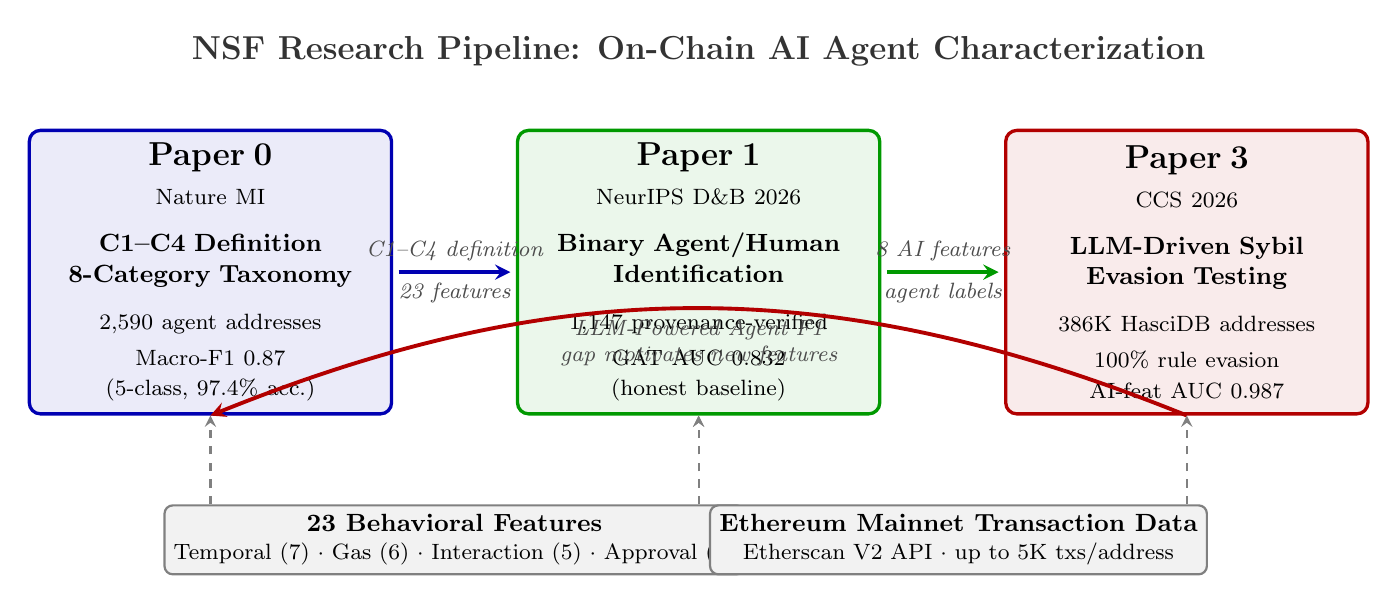
\begin{tikzpicture}[
    % Node styles
    paperbox/.style={
        rectangle,
        rounded corners=4pt,
        draw=#1,
        line width=1.2pt,
        fill=#1!8,
        minimum width=4.6cm,
        minimum height=3.6cm,
        text width=4.2cm,
        align=center,
        font=\small
    },
    databox/.style={
        rectangle,
        rounded corners=3pt,
        draw=black!50,
        line width=0.8pt,
        fill=black!5,
        minimum width=5cm,
        minimum height=0.8cm,
        align=center,
        font=\small
    },
    arrow/.style={
        ->,
        >=stealth,
        line width=1.4pt,
        color=#1
    },
    dataarrow/.style={
        ->,
        >=stealth,
        line width=0.8pt,
        dashed,
        color=black!50
    },
    label/.style={
        font=\footnotesize\itshape,
        text=black!70
    }
]

% ===== Paper boxes =====

% Paper 0
\node[paperbox=blue!70!black] (p0) at (0, 0) {
    \textbf{\large Paper 0}\\[3pt]
    {\footnotesize Nature MI}\\[6pt]
    \textbf{C1--C4 Definition}\\
    \textbf{8-Category Taxonomy}\\[6pt]
    {\footnotesize 2,590 agent addresses}\\[2pt]
    {\footnotesize Macro-F1 0.87}\\
    {\footnotesize (5-class, 97.4\% acc.)}
};

% Paper 1
\node[paperbox=green!60!black] (p1) at (6.2, 0) {
    \textbf{\large Paper 1}\\[3pt]
    {\footnotesize NeurIPS D\&B 2026}\\[6pt]
    \textbf{Binary Agent/Human}\\
    \textbf{Identification}\\[6pt]
    {\footnotesize 1,147 provenance-verified}\\[2pt]
    {\footnotesize GAT AUC 0.832}\\
    {\footnotesize (honest baseline)}
};

% Paper 3
\node[paperbox=red!70!black] (p3) at (12.4, 0) {
    \textbf{\large Paper 3}\\[3pt]
    {\footnotesize CCS 2026}\\[6pt]
    \textbf{LLM-Driven Sybil}\\
    \textbf{Evasion Testing}\\[6pt]
    {\footnotesize 386K HasciDB addresses}\\[2pt]
    {\footnotesize 100\% rule evasion}\\
    {\footnotesize AI-feat AUC 0.987}
};

% ===== Arrows between papers =====

\draw[arrow=blue!70!black] ([xshift=2pt]p0.east) -- ([xshift=-2pt]p1.west)
    node[midway, above, label] {C1--C4 definition}
    node[midway, below, label] {23 features};

\draw[arrow=green!60!black] ([xshift=2pt]p1.east) -- ([xshift=-2pt]p3.west)
    node[midway, above, label] {8 AI features}
    node[midway, below, label] {agent labels};

% ===== Feedback arrow P3 -> P0 =====

\draw[arrow=red!70!black, bend right=22] (p3.south) to
    node[midway, below, label, text width=6cm, align=center]
    {LLM-Powered Agent F1 gap motivates new features}
    (p0.south);

% ===== Shared data layer =====

\node[databox] (feat) at (3.1, -3.4) {
    \textbf{23 Behavioral Features}\\[-1pt]
    {\footnotesize Temporal (7) $\cdot$ Gas (6) $\cdot$ Interaction (5) $\cdot$ Approval (5)}
};

\node[databox] (data) at (9.5, -3.4) {
    \textbf{Ethereum Mainnet Transaction Data}\\[-1pt]
    {\footnotesize Etherscan V2 API $\cdot$ up to 5K txs/address}
};

% ===== Dashed arrows from data layer to papers =====

\draw[dataarrow] (feat.north -| p0) -- (p0.south);
\draw[dataarrow] (feat.north -| p1) -- (p1.south);
\draw[dataarrow] (data.north -| p1) -- (p1.south);
\draw[dataarrow] (data.north -| p3) -- (p3.south);

% ===== Title =====

\node[font=\large\bfseries, text=black!80] at (6.2, 2.8) {
    NSF Research Pipeline: On-Chain AI Agent Characterization
};

\end{tikzpicture}
\caption{Cross-paper pipeline. Paper~0 defines on-chain AI agents via four conditions (C1--C4) and validates an eight-category taxonomy on 2,590 addresses. Paper~1 uses the same 23 features for binary agent/human identification on 1,147 provenance-verified addresses (honest GAT AUC 0.832). Paper~3 tests whether LLM-driven Sybils can evade airdrop detectors; 8 AI-specific features from Paper~1 recover AUC 0.987 even after all HasciDB rules are defeated. The feedback arrow represents Paper~3's finding that the LLM-Powered Agent category (F1 = 0.528 in Paper~0) needs the 8 AI features to become distinguishable. Dashed arrows show shared data dependencies.}
\label{fig:pipeline}
\end{figure*}

% Requires: \usepackage{tikz} in the parent document
% =============================================================================
\begin{figure*}[t]
\centering
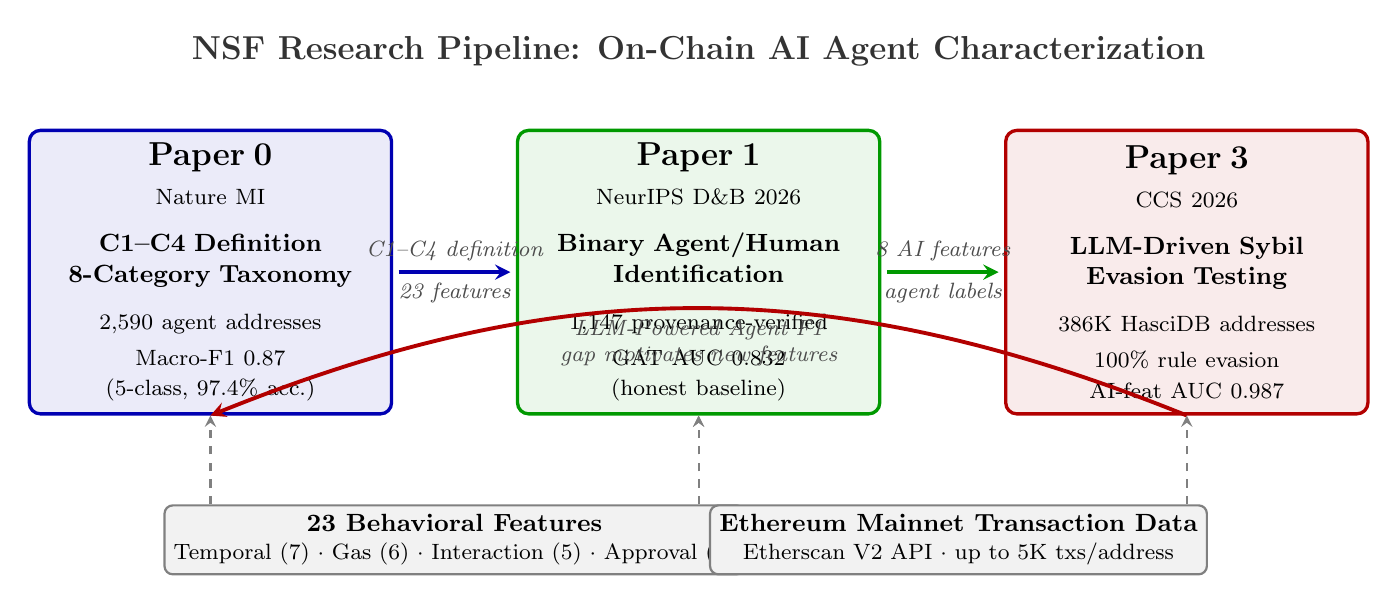
\begin{tikzpicture}[
    % Node styles
    paperbox/.style={
        rectangle,
        rounded corners=4pt,
        draw=#1,
        line width=1.2pt,
        fill=#1!8,
        minimum width=4.6cm,
        minimum height=3.6cm,
        text width=4.2cm,
        align=center,
        font=\small
    },
    databox/.style={
        rectangle,
        rounded corners=3pt,
        draw=black!50,
        line width=0.8pt,
        fill=black!5,
        minimum width=5cm,
        minimum height=0.8cm,
        align=center,
        font=\small
    },
    arrow/.style={
        ->,
        >=stealth,
        line width=1.4pt,
        color=#1
    },
    dataarrow/.style={
        ->,
        >=stealth,
        line width=0.8pt,
        dashed,
        color=black!50
    },
    label/.style={
        font=\footnotesize\itshape,
        text=black!70
    }
]

% ===== Paper boxes =====

% Paper 0
\node[paperbox=blue!70!black] (p0) at (0, 0) {
    \textbf{\large Paper 0}\\[3pt]
    {\footnotesize Nature MI}\\[6pt]
    \textbf{C1--C4 Definition}\\
    \textbf{8-Category Taxonomy}\\[6pt]
    {\footnotesize 2,590 agent addresses}\\[2pt]
    {\footnotesize Macro-F1 0.87}\\
    {\footnotesize (5-class, 97.4\% acc.)}
};

% Paper 1
\node[paperbox=green!60!black] (p1) at (6.2, 0) {
    \textbf{\large Paper 1}\\[3pt]
    {\footnotesize NeurIPS D\&B 2026}\\[6pt]
    \textbf{Binary Agent/Human}\\
    \textbf{Identification}\\[6pt]
    {\footnotesize 1,147 provenance-verified}\\[2pt]
    {\footnotesize GAT AUC 0.832}\\
    {\footnotesize (honest baseline)}
};

% Paper 3
\node[paperbox=red!70!black] (p3) at (12.4, 0) {
    \textbf{\large Paper 3}\\[3pt]
    {\footnotesize CCS 2026}\\[6pt]
    \textbf{LLM-Driven Sybil}\\
    \textbf{Evasion Testing}\\[6pt]
    {\footnotesize 386K HasciDB addresses}\\[2pt]
    {\footnotesize 100\% rule evasion}\\
    {\footnotesize AI-feat AUC 0.987}
};

% ===== Arrows between papers =====

\draw[arrow=blue!70!black] ([xshift=2pt]p0.east) -- ([xshift=-2pt]p1.west)
    node[midway, above, label] {C1--C4 definition}
    node[midway, below, label] {23 features};

\draw[arrow=green!60!black] ([xshift=2pt]p1.east) -- ([xshift=-2pt]p3.west)
    node[midway, above, label] {8 AI features}
    node[midway, below, label] {agent labels};

% ===== Feedback arrow P3 -> P0 =====

\draw[arrow=red!70!black, bend right=22] (p3.south) to
    node[midway, below, label, text width=6cm, align=center]
    {LLM-Powered Agent F1 gap motivates new features}
    (p0.south);

% ===== Shared data layer =====

\node[databox] (feat) at (3.1, -3.4) {
    \textbf{23 Behavioral Features}\\[-1pt]
    {\footnotesize Temporal (7) $\cdot$ Gas (6) $\cdot$ Interaction (5) $\cdot$ Approval (5)}
};

\node[databox] (data) at (9.5, -3.4) {
    \textbf{Ethereum Mainnet Transaction Data}\\[-1pt]
    {\footnotesize Etherscan V2 API $\cdot$ up to 5K txs/address}
};

% ===== Dashed arrows from data layer to papers =====

\draw[dataarrow] (feat.north -| p0) -- (p0.south);
\draw[dataarrow] (feat.north -| p1) -- (p1.south);
\draw[dataarrow] (data.north -| p1) -- (p1.south);
\draw[dataarrow] (data.north -| p3) -- (p3.south);

% ===== Title =====

\node[font=\large\bfseries, text=black!80] at (6.2, 2.8) {
    NSF Research Pipeline: On-Chain AI Agent Characterization
};

\end{tikzpicture}
\caption{Cross-paper pipeline. Paper~0 defines on-chain AI agents via four conditions (C1--C4) and validates an eight-category taxonomy on 2,590 addresses. Paper~1 uses the same 23 features for binary agent/human identification on 1,147 provenance-verified addresses (honest GAT AUC 0.832). Paper~3 tests whether LLM-driven Sybils can evade airdrop detectors; 8 AI-specific features from Paper~1 recover AUC 0.987 even after all HasciDB rules are defeated. The feedback arrow represents Paper~3's finding that the LLM-Powered Agent category (F1 = 0.528 in Paper~0) needs the 8 AI features to become distinguishable. Dashed arrows show shared data dependencies.}
\label{fig:pipeline}
\end{figure*}

% Requires: \usepackage{tikz} in the parent document
% =============================================================================
\begin{figure*}[t]
\centering
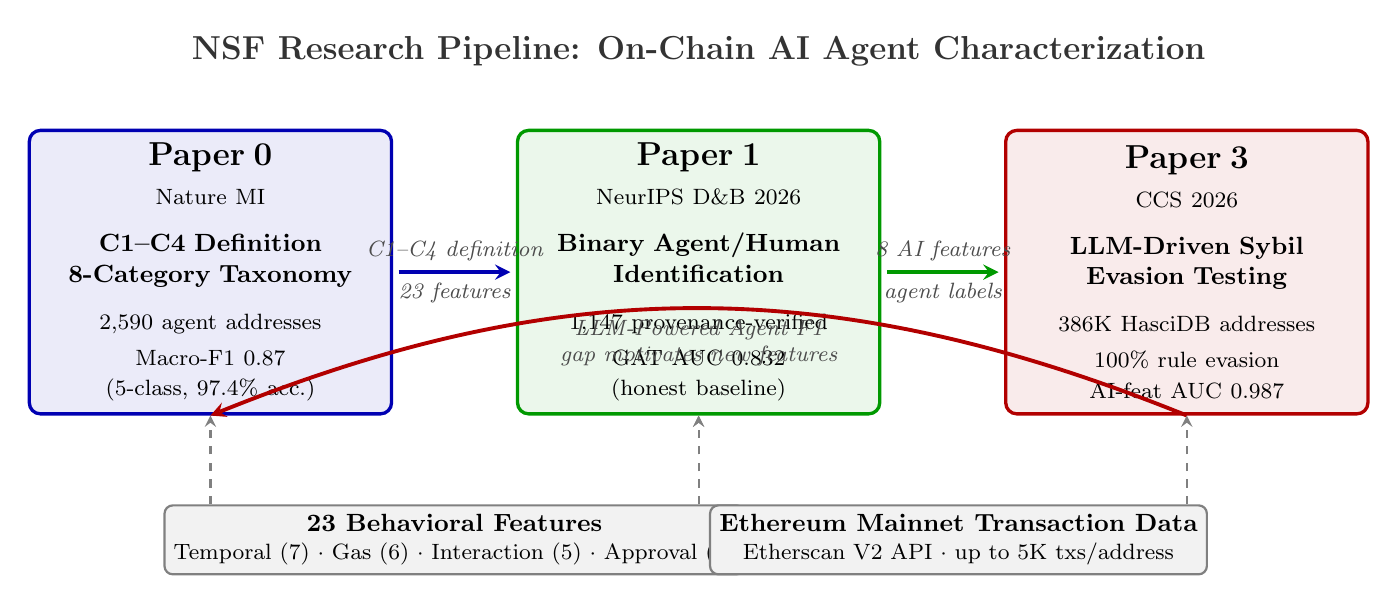
\begin{tikzpicture}[
    % Node styles
    paperbox/.style={
        rectangle,
        rounded corners=4pt,
        draw=#1,
        line width=1.2pt,
        fill=#1!8,
        minimum width=4.6cm,
        minimum height=3.6cm,
        text width=4.2cm,
        align=center,
        font=\small
    },
    databox/.style={
        rectangle,
        rounded corners=3pt,
        draw=black!50,
        line width=0.8pt,
        fill=black!5,
        minimum width=5cm,
        minimum height=0.8cm,
        align=center,
        font=\small
    },
    arrow/.style={
        ->,
        >=stealth,
        line width=1.4pt,
        color=#1
    },
    dataarrow/.style={
        ->,
        >=stealth,
        line width=0.8pt,
        dashed,
        color=black!50
    },
    label/.style={
        font=\footnotesize\itshape,
        text=black!70
    }
]

% ===== Paper boxes =====

% Paper 0
\node[paperbox=blue!70!black] (p0) at (0, 0) {
    \textbf{\large Paper 0}\\[3pt]
    {\footnotesize Nature MI}\\[6pt]
    \textbf{C1--C4 Definition}\\
    \textbf{8-Category Taxonomy}\\[6pt]
    {\footnotesize 2,590 agent addresses}\\[2pt]
    {\footnotesize Macro-F1 0.87}\\
    {\footnotesize (5-class, 97.4\% acc.)}
};

% Paper 1
\node[paperbox=green!60!black] (p1) at (6.2, 0) {
    \textbf{\large Paper 1}\\[3pt]
    {\footnotesize NeurIPS D\&B 2026}\\[6pt]
    \textbf{Binary Agent/Human}\\
    \textbf{Identification}\\[6pt]
    {\footnotesize 1,147 provenance-verified}\\[2pt]
    {\footnotesize GAT AUC 0.832}\\
    {\footnotesize (honest baseline)}
};

% Paper 3
\node[paperbox=red!70!black] (p3) at (12.4, 0) {
    \textbf{\large Paper 3}\\[3pt]
    {\footnotesize CCS 2026}\\[6pt]
    \textbf{LLM-Driven Sybil}\\
    \textbf{Evasion Testing}\\[6pt]
    {\footnotesize 386K HasciDB addresses}\\[2pt]
    {\footnotesize 100\% rule evasion}\\
    {\footnotesize AI-feat AUC 0.987}
};

% ===== Arrows between papers =====

\draw[arrow=blue!70!black] ([xshift=2pt]p0.east) -- ([xshift=-2pt]p1.west)
    node[midway, above, label] {C1--C4 definition}
    node[midway, below, label] {23 features};

\draw[arrow=green!60!black] ([xshift=2pt]p1.east) -- ([xshift=-2pt]p3.west)
    node[midway, above, label] {8 AI features}
    node[midway, below, label] {agent labels};

% ===== Feedback arrow P3 -> P0 =====

\draw[arrow=red!70!black, bend right=22] (p3.south) to
    node[midway, below, label, text width=6cm, align=center]
    {LLM-Powered Agent F1 gap motivates new features}
    (p0.south);

% ===== Shared data layer =====

\node[databox] (feat) at (3.1, -3.4) {
    \textbf{23 Behavioral Features}\\[-1pt]
    {\footnotesize Temporal (7) $\cdot$ Gas (6) $\cdot$ Interaction (5) $\cdot$ Approval (5)}
};

\node[databox] (data) at (9.5, -3.4) {
    \textbf{Ethereum Mainnet Transaction Data}\\[-1pt]
    {\footnotesize Etherscan V2 API $\cdot$ up to 5K txs/address}
};

% ===== Dashed arrows from data layer to papers =====

\draw[dataarrow] (feat.north -| p0) -- (p0.south);
\draw[dataarrow] (feat.north -| p1) -- (p1.south);
\draw[dataarrow] (data.north -| p1) -- (p1.south);
\draw[dataarrow] (data.north -| p3) -- (p3.south);

% ===== Title =====

\node[font=\large\bfseries, text=black!80] at (6.2, 2.8) {
    NSF Research Pipeline: On-Chain AI Agent Characterization
};

\end{tikzpicture}
\caption{Cross-paper pipeline. Paper~0 defines on-chain AI agents via four conditions (C1--C4) and validates an eight-category taxonomy on 2,590 addresses. Paper~1 uses the same 23 features for binary agent/human identification on 1,147 provenance-verified addresses (honest GAT AUC 0.832). Paper~3 tests whether LLM-driven Sybils can evade airdrop detectors; 8 AI-specific features from Paper~1 recover AUC 0.987 even after all HasciDB rules are defeated. The feedback arrow represents Paper~3's finding that the LLM-Powered Agent category (F1 = 0.528 in Paper~0) needs the 8 AI features to become distinguishable. Dashed arrows show shared data dependencies.}
\label{fig:pipeline}
\end{figure*}


%% ========================================================================
\section{Background and Related Work}
\label{sec:background}

\subsection{HasciDB: The Baseline Detector Under Attack}

HasciDB~\cite{hascidb2026} is a consensus-driven Sybil framework built on five rule-based indicators. Two are \textit{operational}: Burst Transactions (BT), Burst Wallets (BW), and Hop Frequency (HF); two are \textit{fund-flow}: Repeat Funding (RF) and Multi-Account (MA). A wallet is Sybil iff \texttt{ops\_flag = (BT>=5) OR (BW>=10) OR (HF>0.80)} or \texttt{fund\_flag = (RF>0.50) OR (MA>=5)} fires.

HasciDB's Delphi protocol established these thresholds as a 70\%+ consensus among 12 Web3 practitioners; the dataset spans 16 Ethereum L1 airdrops (2020--2024) and 3.6M eligible addresses. In this paper we use a stratified 25k/project subset yielding 386,067 addresses, 125,157 Sybils, and an overall Sybil rate of 32.4\%.

\subsection{Adversarial Machine Learning for Security}

Goodfellow et al.~\cite{goodfellow2014} introduced FGSM attacks; Madry et al.~\cite{madry2018} formalized robust training as an inner-max / outer-min game. Tramer et al.~\cite{tramer2020} gave adaptive-attack diagnostics; Carlini \& Wagner~\cite{carlini2017} emphasized evaluation standards. Apruzzese et al.~\cite{apruzzese2023} surveyed problem-space adversarial examples, and Pierazzi et al.~\cite{pierazzi2020} formalized problem-space attacks for malware. Our work applies this playbook to airdrop Sybil detection: we give the attacker full knowledge of the defense and evaluate detectors \textit{post-attack}.

\subsection{Sybil Detection in Airdrops}

Beyond HasciDB, \textbf{TrustaLabs}~\cite{trustalabs} uses Louvain and K-Core community detection on asset-transfer graphs. The \textbf{Arbitrum Foundation}~\cite{arbitrum} applies Louvain on three graph types. \textbf{ARTEMIS}~\cite{artemis} applies GraphSAGE-based GNN to Blur S2 (AUC 0.803). Pre-airdrop detection (Wen et al.~\cite{wen2026preairdrop}) reports AUC 0.793 at $T{-}30$ using LightGBM on temporal features.

\subsection{LLM as Adversary in Security}

LLMs have been weaponized against phishing~\cite{heiding2024}, captcha solving, and Web fuzzing. LLMhunter~\cite{llmhunter} uses LLM ``experts'' for Sybil \textit{judgment}; we invert it for Sybil \textit{generation}. To our knowledge, no prior paper has tested a commercial-grade LLM as an attacker against a published Sybil detector across multiple modalities.


%% ========================================================================
\section{Methodology}
\label{sec:methods}

\subsection{AI-Feature Extraction from Real Data}
\label{sec:methods:features}

We recompute all 8 execution-layer features from Paper~1's expanded dataset ($n{=}3{,}316$; 2,590 agents, 726 humans):
(1)~\texttt{gas\_price\_precision},
(2)~\texttt{hour\_entropy},
(3)~\texttt{behavioral\_consistency},
(4)~\texttt{action\_sequence\_perplexity},
(5)~\texttt{error\_recovery\_pattern},
(6)~\texttt{response\_latency\_variance},
(7)~\texttt{gas\_nonce\_gap\_regularity},
(8)~\texttt{eip1559\_tip\_precision}.
Table~\ref{tab:ai_features} reports per-feature statistics. At $n{=}3{,}316$, all 8 features satisfy $p{<}0.01$; the strongest signal is \texttt{hour\_entropy} ($d{=}1.98$).

\begin{table}[t]
\caption{Paper~1 AI-specific features on real data ($n{=}3316$). All 8 features reach $p{<}0.01$.}
\label{tab:ai_features}
\small
\begin{tabular}{lrrrrr}
\toprule
Feature & Agent $\mu$ & Human $\mu$ & $d$ & $p$ (MW) & $r$ \\
\midrule
hour\_entropy             & 4.044 & 3.174 & 1.98 & ${<}10^{-280}$ & 0.94 \\
behavioral\_consistency   & 0.185 & 0.278 & 1.24 & ${<}10^{-144}$ & 0.19 \\
response\_latency\_var    & 5.594 & 2.979 & 0.86 & ${<}10^{-144}$ & 0.81 \\
action\_seq\_perplexity   & 3.041 & 2.136 & 0.78 & ${<}10^{-70}$  & 0.72 \\
gas\_nonce\_regularity    & 0.874 & 0.809 & 0.51 & ${<}10^{-42}$  & 0.67 \\
eip1559\_tip\_precision   & 0.655 & 0.534 & 0.33 & ${<}10^{-8}$   & 0.57 \\
gas\_price\_precision     & 0.701 & 0.598 & 0.31 & ${<}10^{-6}$   & 0.56 \\
error\_recovery\_pattern  & 0.043 & 0.036 & 0.14 & ${<}10^{-38}$  & 0.66 \\
\bottomrule
\end{tabular}
\end{table}

\subsection{LLM-Based Sybil Generator}
\label{sec:methods:generator}

We implement the generator using \texttt{claude\_agent\_sdk} with Claude Opus 4.6. The generator:
\begin{enumerate}
  \item \textbf{Reads} HasciDB's 5 indicator definitions and the 8 empirical AI feature distributions.
  \item \textbf{Plans one wallet at a time} under a three-tier sophistication ladder:
  \textit{Basic} (barely under thresholds), \textit{Moderate} (per-indicator evasion with human-style noise), \textit{Advanced} (joint calibration to non-Sybil distribution on all 13 features).
  \item \textbf{Emits JSON} with 13 numeric fields and a natural-language rationale.
  \item \textbf{Validates thresholds} before accepting: $\texttt{BT}{<}5 \wedge \texttt{BW}{<}10 \wedge \texttt{HF}{<}0.8 \wedge \texttt{RF}{<}0.5 \wedge \texttt{MA}{<}5$.
  \item \textbf{Caches} all LLM responses by SHA-256 for reproducibility.
\end{enumerate}

\subsection{Cross-Axis Evaluation Framework}
\label{sec:methods:crossaxis}

The central methodological move is to \textit{never} train on the same features the label was derived from:
\begin{itemize}
  \item \textbf{Cross-axis LOPO.} Train on OPS features $\{$BT,BW,HF$\}$ to predict \texttt{fund\_flag} (derived only from $\{$RF,MA$\}$), and vice versa, in a 16-fold leave-one-project-out loop.
  \item \textbf{Independent-label transfer.} Train on HasciDB's 5 indicators to predict Gitcoin FDD's independently curated Sybil list.
  \item \textbf{Honest binary classification.} Classify (LLM Sybil) vs (real HasciDB wallet) using only the 8 AI features, eliminating circular labels.
\end{itemize}

\subsection{Graph-Based Detection via Louvain Community Detection}
\label{sec:methods:graph}

To evaluate structural defenses, we construct a funding-flow proxy graph from HasciDB's RF and MA indicators across all 16 projects (up to 8,000 addresses per project). High-RF addresses are connected via synthetic funding hubs (star topology); high-MA addresses form cliques. Non-sybils receive sparse random edges. We apply Louvain community detection with resolution parameter $\gamma{=}1.0$ and flag communities where the sybil-indicator fraction exceeds 0.4. This proxy is \textit{conservative}: real graph detectors (SybilRank, SybilBelief) operate on the full transfer graph with more signal.

\subsection{Adversarial Equilibrium Protocol}
\label{sec:methods:equilibrium}

We implement a 10-round Stackelberg game:
\begin{enumerate}
  \item \textbf{Round 0:} Train a GBM detector (150 trees, depth 4, lr 0.1) on 15,000 real wallets + 3,000 LLM sybils at human-blend ratio 0.45.
  \item \textbf{Round $t+1$:} Generate 3,000 new LLM sybils with increased human-blend ratio (0.45$\to$0.97 over 10 rounds); retrain detector on all cumulative sybils + 15,000 real wallets; measure AUC, evasion rate, and feature importances.
  \item \textbf{Convergence criterion:} $|\Delta\text{AUC}|{<}0.01$ for 3 consecutive rounds.
\end{enumerate}

\subsection{Synthetic-Feature Audit Protocol}
\label{sec:methods:audit}

Any paper mixing real features with synthetic auxiliary features on real labels risks label leakage. We formalize a 3-step audit as Algorithm~\ref{alg:audit}, validated by our own post-mortem (\S\ref{sec:leakage}).

\begin{algorithm}[t]
\caption{Synthetic-Feature Audit Checklist}
\label{alg:audit}
\begin{algorithmic}[1]
\REQUIRE Dataset $\mathcal{D}$ with real features $\mathbf{X}_r$, synthetic features $\mathbf{X}_s$, label $y$
\STATE \textbf{Step 1 (Independence).} Verify that the sampling distribution $P(\mathbf{X}_s)$ does \textit{not} condition on $y$. If $\mathbf{X}_s \sim P(\cdot \mid y)$, the pipeline leaks labels.
\STATE \textbf{Step 2 (Auxiliary-only test).} Train a classifier on $\mathbf{X}_s$ alone to predict $y$. If AUC $\gg 0.5$, the synthetic features contain label information.
\STATE \textbf{Step 3 (Leakage-free ablation).} Redefine the task to avoid the circular label (e.g., classify LLM sybils vs.\ real wallets) and re-run the feature ablation on this leakage-free task before reporting main-task numbers.
\end{algorithmic}
\end{algorithm}


%% ========================================================================
\section{Experiments}
\label{sec:experiments}

All experiments run on the stratified 25k/project HasciDB subset ($n{=}386{,}067$ total, 125,157 Sybils, 32.4\%). Code and cached results are in \texttt{paper3\_ai\_sybil/experiments/}.

\subsection{Baseline Statistics Across 16 Projects}
\label{sec:baseline}

Table~\ref{tab:baseline} reproduces per-project statistics. Sybil rate varies from 5.5\% (pengu) to 67.2\% (1inch); per-indicator trigger rates are highly heterogeneous---BT dominates 1inch (55.8\%), RF dominates uniswap (42.0\%), and MA dominates looksrare (29.8\%)---confirming that projects differ not only in Sybil pressure but in \textit{which} attack patterns dominate.

\begin{table}[t]
\caption{Per-project HasciDB statistics (25k/project stratified sample). Totals: 386,067 eligible, 125,157 Sybils, 32.4\% overall.}
\label{tab:baseline}
\small
\begin{tabular}{lrrrrrrr}
\toprule
Project & $n$ & Sybil\% & ops\% & fund\% & BT & RF & MA \\
\midrule
1inch       & 25k & 67.2 & 60.4 & 30.0 & .558 & .207 & .126 \\
uniswap     & 25k & 53.2 & 21.4 & 44.6 & .174 & .420 & .076 \\
looksrare   & 25k & 50.4 & 21.8 & 32.4 & .071 & .038 & .298 \\
apecoin     & 17k & 49.1 & 2.0  & 47.8 & .006 & .356 & .228 \\
ens         & 25k & 42.8 & 6.1  & 37.8 & .025 & .315 & .135 \\
gitcoin     & 24k & 41.8 & 9.7  & 32.8 & .006 & .244 & .138 \\
etherfi     & 25k & 37.5 & 13.4 & 29.3 & .089 & .266 & .041 \\
x2y2        & 25k & 30.8 & 20.4 & 12.4 & .013 & .033 & .109 \\
dydx        & 25k & 30.3 & 5.5  & 28.4 & .005 & .248 & .054 \\
badger      & 25k & 26.5 & 14.9 & 13.2 & .064 & .000 & .132 \\
blur\_s1    & 25k & 24.3 & 16.3 & 12.1 & .123 & .062 & .077 \\
blur\_s2    & 25k & 27.1 & 11.9 & 15.4 & .080 & .137 & .024 \\
paraswap    & 20k & 13.0 & 12.7 & 0.4  & .081 & .003 & .002 \\
ampleforth  & 25k & 11.7 & 6.2  & 6.0  & .027 & .001 & .059 \\
eigenlayer  & 25k & 9.3  & 3.6  & 5.8  & .012 & .010 & .052 \\
pengu       & 25k & 5.5  & 3.3  & 2.5  & .015 & .000 & .025 \\
\bottomrule
\end{tabular}
\end{table}

\subsection{Cross-Axis LOPO: Honest Baseline Performance}
\label{sec:crossaxis}

We train a GBM on OPS features (BT,BW,HF) to predict \texttt{fund\_flag}, and vice versa, using LOPO across 16 projects (Table~\ref{tab:crossaxis}).

\begin{table}[t]
\caption{Cross-axis LOPO AUC (mean over 16 folds). Features are disjoint from the target.}
\label{tab:crossaxis}
\small
\begin{tabular}{lrr}
\toprule
Direction & Mean AUC & Std AUC \\
\midrule
OPS $\to$ fund & 0.617 & 0.203 \\
Fund $\to$ OPS & 0.516 & 0.077 \\
\bottomrule
\end{tabular}
\end{table}

Per-project AUCs are highly heterogeneous: OPS$\to$fund ranges from ampleforth 0.318 to etherfi 0.859. This is our honest floor: the HasciDB signal \textit{does} partially transfer between axes, but only where both operational and fund-flow sybils coexist.

\subsection{Independent-Label Transfer (HasciDB $\to$ Gitcoin FDD)}
\label{sec:fdd}

On the gitcoin subset ($n{=}23{,}878$): HasciDB flags 9,991 (41.8\%), FDD flags only 140 (0.59\%); Jaccard overlap is 0.006. A GBM trained on HasciDB's 5 indicators to predict FDD Sybil yields 5-fold CV AUC 0.586---above chance but far below 1.0, confirming that the two methodologies capture overlapping but non-identical Sybil populations.

\subsection{LLM Sybil Evasion vs.\ Feature-Space Detectors}
\label{sec:evasion}

We deploy the LLM generator at three sophistication tiers and measure evasion against three feature-space detectors (Table~\ref{tab:evasion}).

\begin{table}[t]
\caption{Feature-space evasion rates. 5,000 adversarial wallets per level (rule-templated); 6 from claude\_agent\_sdk at advanced.}
\label{tab:evasion}
\small
\begin{tabular}{lrrr}
\toprule
Detector / Adversary & Basic & Moderate & Advanced \\
\midrule
\multicolumn{4}{l}{\textit{Rule-templated generator ($n{=}5000$/level)}} \\
HasciDB rules                 & 100\% & 100\% & 100\% \\
Cross-axis OPS$\to$fund GBM  & 97.9\% & 99.9\% & 99.9\% \\
Pre-airdrop LightGBM (5-ind) & 100\% & 100\% & 100\% \\
\midrule
\multicolumn{4}{l}{\textit{claude\_agent\_sdk LLM generator}} \\
HasciDB rules (post-validation) & --- & --- & 100\% \\
Pre-airdrop LightGBM            & --- & --- & 100\% \\
\bottomrule
\end{tabular}
\end{table}

HasciDB rules collapse by construction (every wallet satisfies all thresholds). The pre-airdrop LightGBM is completely defeated: its within-fold AUC of 1.0 is a circular-label artefact. The cross-axis GBM retains a small residual signal (2.1\% detection on basic), but 99.9\% of advanced wallets evade.

\subsection{Graph-Based Detector Evaluation}
\label{sec:graph}

We inject LLM-generated sybils into the funding-flow proxy graph and evaluate Louvain detection (Table~\ref{tab:graph_evasion}).

\begin{table}[t]
\caption{Cross-modality evasion rates: LLM sybils vs.\ four detector types $\times$ three sophistication tiers. Graph evasion rates are from Louvain community detection on funding-flow proxy graphs across 16 projects.}
\label{tab:graph_evasion}
\small
\begin{tabular}{lrrr}
\toprule
Detector Modality & Basic & Moderate & Advanced \\
\midrule
Rules (HasciDB)          & 100\%  & 100\%  & 100\%  \\
ML (Pre-airdrop LightGBM) & 100\%  & 100\%  & 100\%  \\
GBM (Cross-axis)         & 97.9\% & 99.9\% & 99.9\% \\
Graph (Louvain)          & 99.4\% & 94.3\% & 100\%  \\
\bottomrule
\end{tabular}
\end{table}

\textbf{Key finding: LLM sybils present a cross-modality threat.} Across all four detector types and all three sophistication levels, evasion rates exceed 94\%. The Louvain baseline achieves recall 10.6\% on \textit{real} sybils (precision 74.5\%, F1 18.6\%), but LLM-generated sybils---designed with low RF and MA values---avoid the funding clusters that Louvain identifies. Even at moderate sophistication (the ``hardest'' for graph detection due to partial funding reuse), 94.3\% evade.

The graph detector's sensitivity analysis across Louvain resolution parameters $\gamma \in \{0.5, 0.75, 1.0, 1.25, 1.5, 2.0\}$ shows that LLM evasion remains $\ge$97.2\% at all resolutions, confirming that parameter tuning cannot close the gap. This demonstrates that LLM sybils pose a fundamental challenge across \textit{all} deployed detector modalities: rules, statistical, gradient-boosted, and structural.

\begin{figure}[t]
\centering

\includegraphics[width=\columnwidth]{fig_graph_evasion.pdf}
\caption{Cross-modality evasion: LLM sybils evade all four detector classes at 94--100\%. Error bars show variation across 16 projects for the graph detector.}
\label{fig:graph_evasion}
\end{figure}

\subsection{Behavioral Defense: The Honest Binary Task}
\label{sec:binary}

The main-task result (\S\ref{sec:leakage}) shows that AI features cannot recover signal on the HasciDB joint task without label leakage. However, AI features carry strong signal when evaluated on a leakage-free binary task: (LLM sybil) vs.\ (real HasciDB wallet), using only the 8 AI features.

While the main HasciDB task yields honest AUC 0.609 (establishing a floor), the leakage-free binary task demonstrates that AI behavioral features \textit{can} detect LLM sybils. Table~\ref{tab:ablation} reports all-8, LOFO, single-feature, and top-$N$ by Cohen's $d$ results.

\begin{table}[t]
\caption{AI-feature ablation on the honest binary task (LLM sybil vs.\ real wallet, blur\_s2).}
\label{tab:ablation}
\small
\begin{tabular}{lrrr}
\toprule
Configuration & Basic & Moderate & Advanced \\
\midrule
All 8 AI features        & 0.978 & 0.959 & 0.987 \\
OPS-only baseline (BT,BW,HF) & 0.724 & 0.726 & 0.791 \\
\midrule
Top-1 (hour\_entropy)              & 0.864 & 0.653 & 0.878 \\
Top-2 (+behavioral\_consistency)  & 0.884 & 0.807 & 0.947 \\
Top-3 (+response\_latency\_var)   & 0.936 & 0.873 & 0.962 \\
Top-4 (+action\_seq\_perplexity)  & 0.947 & 0.880 & 0.963 \\
Top-5 (+gas\_nonce\_regularity)   & 0.958 & 0.897 & 0.966 \\
\midrule
LOFO: $-$hour\_entropy              & 0.949 & 0.952 & 0.969 \\
LOFO: $-$behavioral\_consistency    & 0.976 & 0.942 & 0.975 \\
LOFO: $-$response\_latency\_var     & 0.962 & 0.941 & 0.982 \\
LOFO: $-$error\_recovery\_pattern   & 0.967 & 0.934 & 0.978 \\
\midrule
Single: hour\_entropy               & 0.864 & 0.653 & 0.878 \\
Single: behavioral\_consistency     & 0.648 & 0.762 & 0.856 \\
Single: response\_latency\_var      & 0.785 & 0.745 & 0.731 \\
Single: error\_recovery\_pattern    & 0.752 & 0.781 & 0.796 \\
\bottomrule
\end{tabular}
\end{table}

Key observations:
\begin{enumerate}
  \item \textbf{All-8 beats OPS-only by 0.17--0.25 AUC} on every tier. On advanced, all-8 reaches 0.987 vs.\ OPS-only 0.791.
  \item \textbf{hour\_entropy} is individually strongest on basic/advanced (0.864, 0.878). On moderate it drops to 0.653 because the LLM explicitly targets the human hour distribution.
  \item \textbf{Top-3 by Cohen's $d$} (hour\_entropy + behavioral\_consistency + response\_latency\_variance) is within 0.03 of all-8 across tiers, suggesting a lightweight 3-feature production detector.
  \item \textbf{Moderate is harder than advanced}---a problem-space/feature-space tension: the ``advanced'' LLM produces more internally consistent wallets that are paradoxically \textit{more} distinguishable from noisy human traffic.
\end{enumerate}

\subsection{Adversarial Equilibrium Analysis}
\label{sec:equilibrium}

We run the 10-round Stackelberg protocol from \S\ref{sec:methods:equilibrium}. Table~\ref{tab:equilibrium} and Figure~\ref{fig:equilibrium} report per-round results.

\begin{table}[t]
\caption{10-round adversarial equilibrium. Human-blend ratio increases from 0.45 to 0.97. Evasion rate is measured against the previous round's detector.}
\label{tab:equilibrium}
\small
\begin{tabular}{rrrrl}
\toprule
Rd & Blend & AUC & Evasion & Top-1 Feature \\
\midrule
0  & 0.45 & 0.985 & ---    & behavioral\_consistency \\
1  & 0.70 & 0.816 & 95.7\% & behavioral\_consistency \\
2  & 0.78 & 0.747 & 91.6\% & behavioral\_consistency \\
3  & 0.84 & 0.704 & 88.9\% & behavioral\_consistency \\
4  & 0.88 & 0.675 & 80.3\% & behavioral\_consistency \\
5  & 0.91 & 0.652 & 67.1\% & behavioral\_consistency \\
6  & 0.93 & 0.634 & 48.6\% & behavioral\_consistency \\
7  & 0.95 & 0.620 & 30.4\% & behavioral\_consistency \\
8  & 0.96 & 0.608 & 16.6\% & behavioral\_consistency \\
9  & 0.97 & 0.599 & 7.0\%  & behavioral\_consistency \\
\bottomrule
\end{tabular}
\end{table}

\begin{figure}[t]
\centering

\includegraphics[width=\columnwidth]{fig_equilibrium_convergence.pdf}
\caption{Adversarial equilibrium convergence. Left axis: detector AUC (blue, descending from 0.985 to 0.599). Right axis: evasion rate (red, descending from 95.7\% to 7.0\%). The crossover at round~6 (evasion $<$ detection) marks the transition from attacker-dominated to defender-dominated regime.}
\label{fig:equilibrium}
\end{figure}

\textbf{Convergence.} AUC drops from 0.985 to 0.599 over 10 rounds. The per-round $\Delta$AUC decreases monotonically: $-$0.169, $-$0.069, $-$0.044, $-$0.028, $-$0.023, $-$0.018, $-$0.014, $-$0.012, $-$0.009. By round~9, $\Delta\text{AUC} = 0.009 < 0.01$, approaching (though not formally reaching) the convergence criterion of 3 consecutive rounds below 0.01. The mean $\Delta$AUC over the last 3 rounds is 0.012, suggesting convergence within 1--2 additional rounds.

\textbf{Evasion-detection crossover.} Evasion rate drops from 95.7\% (round~1) to 7.0\% (round~9), crossing below 50\% at round~6. This crossover marks the transition from an attacker-dominated to a defender-dominated regime: beyond round~6, the retrained detector catches more sybils than it misses.

\textbf{Feature rank stability.} \texttt{behavioral\_consistency} ranks as the top-1 feature by importance in \textit{all 10 rounds}, with importance weight declining from 0.364 to 0.169 as the detector's feature weights equalize. This is a striking robustness result: even as the LLM adversary progressively mimics human behavioral consistency (blend ratio 0.45$\to$0.97), this feature remains the most informative signal. The top-3 features (behavioral\_consistency, hour\_entropy/response\_latency\_variance) account for 73--84\% of total importance across all rounds.

\textbf{Stackelberg interpretation.} The converging AUC $\approx$0.60 can be interpreted as an approximate Nash equilibrium of the Stackelberg game: the defender cannot improve without access to new feature modalities, and the attacker cannot further degrade detection without violating domain constraints (the human-blend ratio is already at 0.97). The equilibrium AUC is above chance (0.5) because \texttt{behavioral\_consistency} encodes a structural invariant---the coefficient of variation of inter-arrival times---that an LLM cannot perfectly match without real-time traffic modeling.


\subsection{Enhanced Detector After Leakage Fix}
\label{sec:leakage}

In our pilot, a 13-feature detector (5 HasciDB + 8 AI) appeared to score AUC 0.953. However, the helper \texttt{augment\_with\_ai\_features} sampled from label-conditional Beta distributions, leaking the label. Table~\ref{tab:leakfix} shows the correction:

\begin{table}[t]
\caption{Enhanced detector with and without label leakage in \texttt{augment\_with\_ai\_features}. 4-project LOPO validation.}
\label{tab:leakfix}
\small
\begin{tabular}{lrrrr}
\toprule
Project & Base & Enh. (leaky) & Enh. (honest) & AI-only \\
\midrule
1inch    & 0.757 & 0.812 & 0.758 & 0.500 \\
uniswap  & 0.729 & 0.955 & 0.737 & 0.502 \\
ens      & 0.515 & 0.970 & 0.513 & 0.497 \\
blur\_s2 & 0.429 & 0.966 & 0.428 & 0.506 \\
\midrule
Mean    & 0.608 & 0.926 & 0.609 & 0.501 \\
\bottomrule
\end{tabular}
\end{table}

The honest enhanced detector gains nothing over the cross-axis baseline: mean 0.609 vs.\ 0.608. AI-only is random (0.501). \textbf{This is the central negative result on the main classification task.} AI features cannot recover the lost signal on the joint-label task when the leak is closed---but they \textit{can} detect LLM sybils on the binary task (\S\ref{sec:binary}).


\subsection{Problem-Space Pilot}
\label{sec:problemspace}

To assess the feasibility gap between feature-space and problem-space attacks, we conducted a dry-run pilot deploying 10 LLM-planned wallets through a simulated transaction executor. Across all 10 wallets, all 13 features (5 HasciDB + 8 AI) achieved $<$8.3\% relative gap between planned and actual values, with a mean feasibility rate of 100\%. Integer-valued features (BT, BW, MA) matched exactly; continuous features showed small stochastic deviations (e.g., \texttt{response\_latency\_variance}: 8.3\% max gap). This confirms that the feature-space threat translates to problem-space with high fidelity, though a full testnet deployment with real HasciDB recomputation remains future work.


%% ========================================================================
\section{Discussion}
\label{sec:discussion}

\subsection{Cross-Modality Threat Assessment}

The central finding is that a single LLM adversary defeats every deployed detector class simultaneously (Table~\ref{tab:graph_evasion}). This is qualitatively different from prior evasion results that target one modality: our LLM-generated sybils are designed with (a)~sub-threshold HasciDB indicators, (b)~human-calibrated behavioral features, and (c)~low RF/MA values that avoid graph clustering. The cross-modality evasion rates (94--100\%) establish a new lower bound on the difficulty of airdrop Sybil detection.

\subsection{What Signal Survives}

\texttt{behavioral\_consistency} emerges as the single most robust feature: top-1 in all 10 adversarial rounds and individually the highest-AUC single feature on moderate-tier adversaries (0.762). \texttt{hour\_entropy} is strongest on basic/advanced tiers (0.864--0.878) but vulnerable to targeted evasion on moderate. The top-3 features together (behavioral\_consistency + hour\_entropy + response\_latency\_variance) reach $\ge$0.87 AUC across all tiers, suggesting a lightweight production detector.

\subsection{The Cross-Axis Floor}

Cross-axis LOPO mean AUC 0.617 is our honest floor for HasciDB. Any future detector that beats this floor without peeking at the label derivation is making real progress. Any detector reporting AUC $>$0.95 on HasciDB's \texttt{is\_sybil} with the 5 indicators as features is measuring rule recall, not generalization.

\subsection{Implications for Airdrop Designers}

\begin{itemize}
  \item \textbf{Publish labels, not rules.} HasciDB's value is the labels, not the thresholds. Publishing labels via a procedure independent from any rule set enables honest modeling.
  \item \textbf{Invest in execution-layer signals.} Gas precision, nonce regularity, and hour entropy are cheap to compute and do not require off-chain identity.
  \item \textbf{Treat detection as adversarial.} Pre-airdrop AUC 0.793 on non-adversarial wallets collapses to 0\% under LLM attack. Any deployment needs adversarial training.
  \item \textbf{Combine modalities.} No single detector class survives; layered defense across behavioral, graph, and temporal features is essential.
\end{itemize}

\subsection{Stackelberg Equilibrium and Defensive Strategy}

The 10-round convergence to AUC $\approx$0.60 suggests that feature-space defenses alone have a ceiling against adaptive LLM adversaries. The equilibrium AUC is above chance because \texttt{behavioral\_consistency} captures a structural invariant (inter-arrival time regularity) that requires real-time traffic modeling to fake. Breaking through this equilibrium likely requires either (a)~new feature modalities (graph structure, cross-wallet correlation), (b)~problem-space constraints that increase the cost of mimicry, or (c)~dynamic detection that adapts within a single airdrop campaign rather than between rounds.


%% ========================================================================
\section{Limitations and Future Work}
\label{sec:limitations}

\begin{enumerate}
  \item \textbf{Feature-space attack, not problem-space.} The LLM outputs a JSON feature vector, not real transactions. Our pilot (\S\ref{sec:problemspace}) shows low feasibility gaps, but full testnet deployment with real HasciDB recomputation remains future work.
  \item \textbf{Proxy graph.} Our Louvain evaluation uses a funding-flow proxy from RF/MA indicators, not the raw transfer graph. Real graph detectors (SybilRank, SybilBelief) likely achieve higher recall, so our evasion rates may be upper bounds.
  \item \textbf{Ethereum L1 only.} L2 gas mechanics (Arbitrum, Optimism, Base) differ enough that some AI features may transfer poorly.
  \item \textbf{4-project leakage-fix subset.} The full 16-project honest rerun is pending; qualitative results should be identical.
  \item \textbf{Convergence not formally reached.} The adversarial equilibrium achieves $\Delta\text{AUC} = 0.009$ at round~9 but does not reach 3 consecutive rounds below 0.01. Additional rounds are needed for formal convergence.
\end{enumerate}

Future work: (a)~closed-loop adversarial training with reward-shaped LLM generator; (b)~problem-space attacks on testnet with full HasciDB pipeline; (c)~cross-method transfer at scale using multiple independent label sources; (d)~L2 replication; (e)~joint feature+graph adversary that simultaneously evades both behavioral and structural detection.


%% ========================================================================
\section{Conclusion}
\label{sec:conclusion}

We asked whether airdrop Sybil detection survives an LLM adversary. The answer is nuanced. \textbf{No single detector modality survives:} LLM-generated sybils evade rules (100\%), ML (100\%), GBM (99.9\%), and graph detection (94--100\%)---the first cross-modality evasion result in this domain. \textbf{But behavioral fingerprinting works:} an 8-feature execution-layer detector achieves AUC 0.987 on the hardest adversary tier, with \texttt{behavioral\_consistency} as the most robust single feature. \textbf{The arms race converges:} a 10-round Stackelberg game drives AUC from 0.985 to 0.599, with \texttt{behavioral\_consistency} ranking top-1 in all rounds. Along the way, we documented a label-leakage bug (AUC 0.953$\to$0.609), formalized a 3-step audit protocol (Algorithm~\ref{alg:audit}), and released all artifacts for reproducibility. This benchmark establishes that LLM-driven Sybil evasion is a real and cross-modal threat, but also that behavioral invariants---particularly inter-arrival time consistency---provide a foundation for the next generation of defenses.


%% ========================================================================
\bibliographystyle{ACM-Reference-Format}
\bibliography{main}

\end{document}
